% Created 2021-01-02 Sa 03:22
% Intended LaTeX compiler: pdflatex
\documentclass[a4paper]{article}
\usepackage[utf8]{inputenc}
\usepackage[T1]{fontenc}
\usepackage{graphicx}
\usepackage{grffile}
\usepackage{longtable}
\usepackage{wrapfig}
\usepackage{rotating}
\usepackage[normalem]{ulem}
\usepackage{amsmath}
\usepackage{textcomp}
\usepackage{amssymb}
\usepackage{capt-of}
\usepackage{hyperref}
\affiliation{<Your school, think tank, etc>}
\shorttitle{<A short version of the long title for page headers>}
\usepackage{breakcites}
\usepackage{apacite}
\usepackage{paralist}
\let\itemize\compactitem
\let\description\compactdesc
\let\enumerate\compactenum
\author{Vignesh Gopinathan Ali Rida Bahja Amr Elsayed}
\date{\today}
\title{Chapter 3}
\hypersetup{
 pdfauthor={Vignesh Gopinathan Ali Rida Bahja Amr Elsayed},
 pdftitle={Chapter 3},
 pdfkeywords={},
 pdfsubject={},
 pdfcreator={Emacs 26.3 (Org mode 9.4)}, 
 pdflang={English}}
\begin{document}

\maketitle
\tableofcontents

\begin{ABSTRACT}
\textbf{Abstract}
\end{ABSTRACT}
\tableofcontents
\section{Histogram procesing}
\label{sec:orgaa70f41}
we represent pictures using M x N pixels and each pixel has an integer value.
Histogram is a graphical representation of the intensity distribution of an image.
In simple terms, it represents the number of pixels for each intensity value considered.
\subsection{Histogram Example}
\label{sec:org0b3cc87}
xxx change the picture with picture and histogram of it
\begin{center}
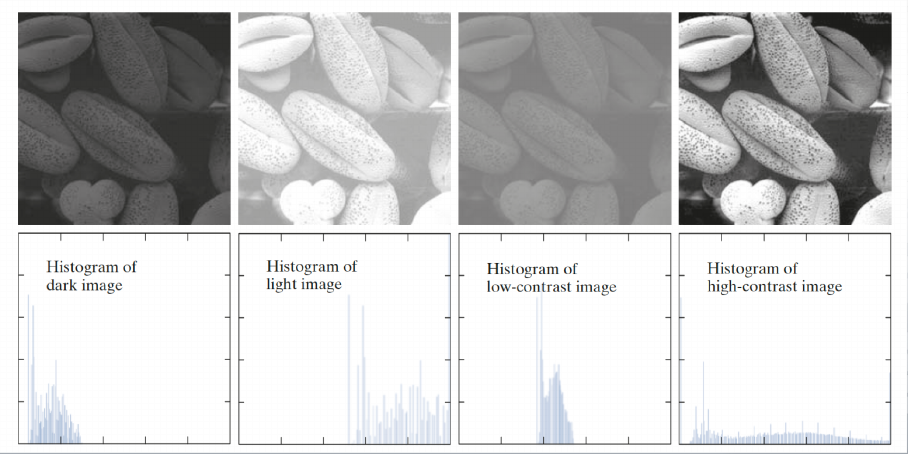
\includegraphics[angle=0,width=9cm]{./img/histogram_example.png}
\end{center}
In the above figure, X-axis represents the tonal scale (black at the left and white at the right),
and Y-axis represents the number of pixels in an image. Here,
the histogram shows the number of pixels for each brightness level (from black to white),
and when there are more pixels, the peak at the certain brightness level is higher.

\subsection{Histogram equalization}
\label{sec:orgc969886}
xxx In this section we will talk about histogram equalization.

Histogram Equalization is a computer image processing technique used to improve contrast in images.
It accomplishes this by effectively spreading out the most frequent intensity values,
i.e. stretching out the intensity range of the image.
This method usually increases the global contrast of images when its usable data is represented by close contrast values.
This allows for areas of lower local contrast to gain a higher contrast.

we used python code [Histo.py] to represent the idea.
\begin{figure}[htbp]
\centering
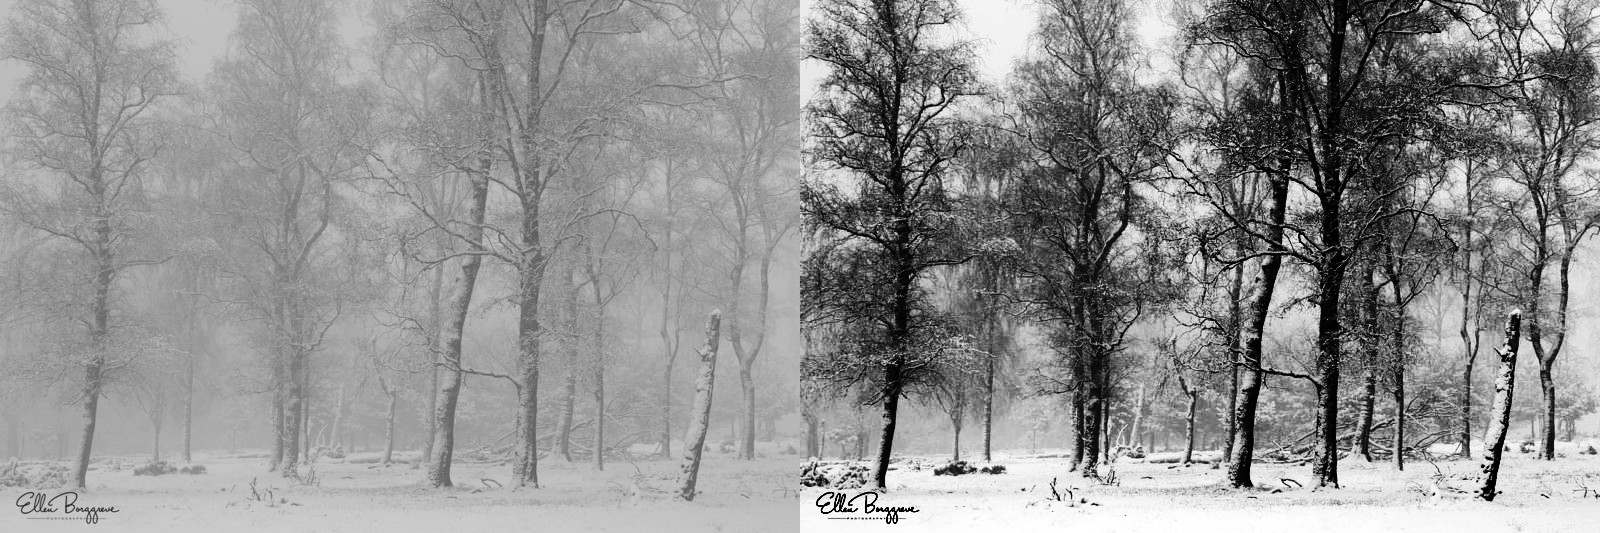
\includegraphics[angle=0,width=9cm]{./img/res.png}
\caption{\label{result of histogram equalization}Example on the importance of histograms}
\end{figure}

A color histogram of an image represents the number of pixels in each type of color component.
Histogram equalization cannot be applied separately to the Red, Green and Blue components of the image as
it leads to dramatic changes in the image’s color balance.
However, if the image is first converted to another color space, like HSL/HSV color space,
then the algorithm can be applied to the luminance or value channel without
resulting in changes to the hue and saturation of the image.
\section{Fundamentals of spatial filtering}
\label{sec:org27a6e22}
The name filter is borrowed from frequency domain processing where “filtering” refers to passing, modifying,
or rejecting specified frequency components of an image. For example, a filter that passes low frequencies is called a lowpass filter.
The net effect produced by a lowpass filter is to smooth an image by blurring it. We can accomplish similar smoothing directly on the
image itself by using spatial filters.
Spatial filtering modifies an image by replacing the value of each pixel by a function of the values of the pixel and its neighbors. If the
operation performed on the image pixels is linear, then the filter is called a linear spatial filter. Otherwise, the filter is a nonlinear spatial
filter. We will focus attention first on linear filters and then introduce some basic nonlinear filters. 
\subsection{linear filtering}
\label{sec:org98fddc8}
kernel
\subsection{image padding}
\label{sec:org7f7d75c}
\subsection{correlation and convolution}
\label{sec:org6763592}
\subsection{Gaussian Filter}
\label{sec:orgc223ba7}
    A Gaussian filter is a linear filter. It's usually used to blur the image or to reduce noise. If you use two of them and subtract,
    you can use them for "unsharp masking" (edge detection).
    The Gaussian filter alone will blur edges and reduce contrast.
The Median filter is a non-linear filter that is most commonly used as a simple way to reduce noise in an image.
It's claim to fame (over Gaussian for noise reduction)
is that it removes noise while keeping edges relatively sharp.
I guess the one advantage a Gaussian filter has over a median filter is that it's faster because multiplying and adding is probably faster than sorting.

\subsubsection{sigma importance}
\label{sec:org619ed11}
I think it should be done in the following steps, first from the signal processing point of view:

\begin{enumerate}
\item Gaussian Filter is a low pass filter. Low pass filters as their names imply pass low frequencies - keeping low frequencies.
\end{enumerate}
So when we look at the image in the frequency domain the highest frequencies happen in the edges
(places that there is a high change in intensity and each intensity value corresponds to a specific visible frequency).
\begin{enumerate}
\item The role of sigma in the Gaussian filter is to control the variation around its mean value.
\end{enumerate}
So as the Sigma becomes larger the more variance allowed around mean and as the Sigma becomes smaller the
less variance allowed around mean.
\begin{enumerate}
\item Filtering in the spatial domain is done through convolution.
\end{enumerate}
it simply means that we apply a kernel on every pixel in the image. The law exists for kernels. Their sum has to be zero.


Now putting all together! When we apply a Gaussian filter to an image,
we are doing a low pass filtering. But as you know this happen in the discrete domain(image pixels).
So we have to quantize our Gaussian filter in order to make a Gaussian kernel. In the quantization step,
as the Gaussian filter(GF) has a small sigma it has the steepest pick.
So the more weights will be focused in the center and the less around it.


In the sense of natural image statistics!
The scientists in this field of studies showed that our vision system is a kind of Gaussian filter in the responses to the images.
see for example take a look at a broad scene! don't pay attention to a specific point!
so you see a broad scene with lots things in it. but the details are not clear!
Now see a specific point in that seen. you see more details that previously you didn't.
This is the Sigma appear here. when you increase the sigma you are looking to the broad scene without paying attention
to the details exits. and when you decrease the value you will get more details.


\section{Codes}
\label{sec:orge68e3f3}

\subsection{Histogram code}
\label{sec:org48be7a5}

\begin{verbatim}
import cv2
import numpy as np
from matplotlib import pyplot as plt

img = cv2.imread('./img/2.jpg',0)

hist,bins = np.histogram(img.flatten(),256,[0,256])
cdf = hist.cumsum()
cdf_normalized = cdf * hist.max()/ cdf.max()

plt.subplot(2,1,1)
plt.plot(cdf_normalized, color = 'b')
plt.hist(img.flatten(),256,[0,256], color = 'r')
plt.xlim([0,256])
plt.legend(('cdf','histogram'), loc = 'upper left')

equ = cv2.equalizeHist(img) 
cdf = equ.cumsum()
cdf_normalized_2 = cdf * hist.max()/ cdf.max()


res = np.hstack((img,equ)) #stacking images side-by-side
cv2.imwrite('./img/equ_res.jpg',equ)
cv2.imwrite('./img/res.png',res)

plt.subplot(2,1,2)
plt.hist(equ.flatten(),256,[0,256], color = 'r')
plt.plot(cdf_normalized_2, color = 'b') #cdf is not right 
plt.xlim([0,256])
plt.show()
\end{verbatim}
\end{document}
